\documentclass[12pt]{report}
\usepackage[utf8]{inputenc}
\usepackage[myheadings]{fullpage}

% Package for headers 
\usepackage{fancyhdr}
\usepackage{lastpage}
\usepackage{titlesec}
  
% For figures and stuff
\usepackage{graphicx, wrapfig, subcaption, setspace, booktabs}
\usepackage[T1]{fontenc}

% Change for different font sizes and families
\usepackage[font=small, labelfont=bf]{caption}
\usepackage{fourier}
\usepackage[protrusion=true, expansion=true]{microtype}

%% line and paragraph spacing
% \linespread{1.0}
\setlength{\parskip}{1em}
% \titlespacing{\section}{0pt}{2.5ex plus 1ex minus .2ex}{1.3ex plus .2ex}

% Maths
\usepackage{amsmath,amssymb}
\usepackage{float}
\usepackage{graphicx}
\usepackage{wrapfig}
\usepackage[colorinlistoftodos]{todonotes}
\usepackage[colorlinks=true, allcolors=blue]{hyperref}

% % Bibliography
\usepackage{biblatex} 
\addbibresource{references.bib}

%% Language and font encodings
\usepackage[english]{babel}

% % code
% Better inline directory listings
\usepackage{listings}
\usepackage{xcolor}
\definecolor{light-gray}{gray}{0.95}
\newcommand{\code}[1]{\colorbox{light-gray}{\texttt{#1}}}
\definecolor{codegreen}{rgb}{0,0.6,0}
\definecolor{codegray}{rgb}{0.5,0.5,0.5}
\definecolor{codepurple}{rgb}{0.58,0,0.82}
\definecolor{backcolour}{rgb}{0.95,0.95,0.92}

\lstdefinestyle{mystyle}{
    backgroundcolor=\color{backcolour},   
    commentstyle=\color{codegreen},
    keywordstyle=\color{magenta},
    numberstyle=\tiny\color{codegray},
    stringstyle=\color{codepurple},
    basicstyle=\ttfamily\footnotesize,
    breakatwhitespace=false,         
    breaklines=true,                 
    captionpos=b,                    
    keepspaces=true,                 
    % numbers=left,                    
    % numbersep=5pt,                  
    showspaces=false,                
    showstringspaces=false,
    showtabs=false,                  
    tabsize=4
}

\lstset{style=mystyle}

\newcommand{\HRule}[1]{\rule{\linewidth}{#1}}
\onehalfspacing
\setcounter{tocdepth}{5}
\setcounter{secnumdepth}{5}

%% Sets page size and margins
\usepackage[a4paper,top=2cm,bottom=1.5cm,left=2cm,right=2cm,marginparwidth=1.5cm]{geometry}

% Enable header and footer 
\pagestyle{fancy}
\fancyhf{}

% Header and footer information
\setlength\headheight{15pt}
\fancyhead[L]{ECE 5725 \- Lab3} 
\fancyhead[R]{Yu Zhang\quad}
\fancyfoot[R]{\thepage}

\setlength{\parindent}{0pt} 

\begin{document}

\date{}

% Do not change anything here except in \LARGE \textbf{This is the title of the essay} 
% /hline before and after the title makes those horoziontal lines appear, you can change the appearance by changing the 2pt to different sizees
\title{ \normalsize {\textbf{Cornell University}}
		\\ [1.0cm]
		% Change to your faculty if needed
		
\includegraphics[width=25mm]{img/cornell_logo.png}\\[.5cm]
		Electrical & Computer Engineering \\
		\HRule{2pt} \\
		\LARGE \textbf{ ECE 5725 - Embedded Operating System} \\%para que quede encerrado en las lineas
		\LARGE {\color{blue}{\textbf{LAB3 Report}}}
		\HRule{2pt} \\ [0.5cm]
		\normalsize \ {Lab Section: \textbf{Monday} }\\
% 		\normalsize \today \vspace*{5\baselineskip}
		\normalsize \ {Lab Date: 10/04/21 \And 10/08/21} \vspace*{5\baselineskip}\\
		}
		
\author{
		{ \textbf{Yu Zhang \quad yz2729}}\\[5cm]
		\large {\textbf{\today} } 
		}
		

\maketitle
%\newpage

% Uncomment the next line if you want keywords/index terms after the abstract. 
%\textit{\textbf{Keywords}: lorem, ipsum, dolor}
\section*{1. Introduction\vspace{-1em}}
In this lab, I first learned how to generate the PWM wave with the Raspberry PI and then apply the PWM wave to control DC motors with the Sparkfun TB6612FNG dual-channel motor control. After that, I learned how to assemble a robot platform and control it by designing applications with piTFT.\vspace{-1em} 
\section*{2. Design and Testing\vspace{-1em}}
In this section, I will introduce my experimental process step by step and describe in detail the phenomena and problems I encountered, the solutions and the final results.\vspace{-1em}
\subsection*{2.1 Generate PWM with RPI.GPIO}
The start of this lab is to generate the PWM wave with the Raspberry Pi. I first need to use the Breadboard, a 1K resistor, a red LED and some wires to complete a circuit for testing the PWM wave. \par
Then I designed a python program, \code{blink.py}, to generate the PWM wave. The code is shown in the code listing \ref{code:code1}. I set the GPIO 26 pin in GPIO.OUT mode and initialize it as the source of the PWM wave. Then I configure the frequency as 1 Hz with a duty cycle of 50\%. Apart from this, I also implement an input interface. The user can modify the frequency by inputting a new frequency number. The function \code{ChangeFrequency()} will accept the input and change the frequency of the PWM wave generated by the GPIO 26 pin.\par
\begin{center}
\begin{lstlisting}[language=Python, label=code:code1, caption=blink.py] 
import RPi.GPIO as GPIO
import time 
#setting up gpio pin for pwm
GPIO.setmode(GPIO.BCM)
GPIO.setup(26, GPIO.OUT)
led_pin = GPIO.PWM(26, 1)
led_pin.start(50)
#taking user input to change the frequency of the PWM signal
while(1):
    usr_in = 1
    usr_in = input("Enter a Frequency:")
    led_pin.ChangeFrequency(int(usr_in))
    time.sleep(0.5)
\end{lstlisting}
\end{center}\vspace{-2em}
After connecting the circuit and running the \code{blink.py} program, I successfully found the red LED light connected to the GPIO 26 pin was flashing. What's more, if I inputted a larger frequency, the red LED light would flash faster. This proves that my circuit connection and programming are correct. Besides, I used the PISCOPE to check the generated PWM wave. The result is shown in the figure \ref{fig:figure1}.
\begin{figure}[H]
    \centering
    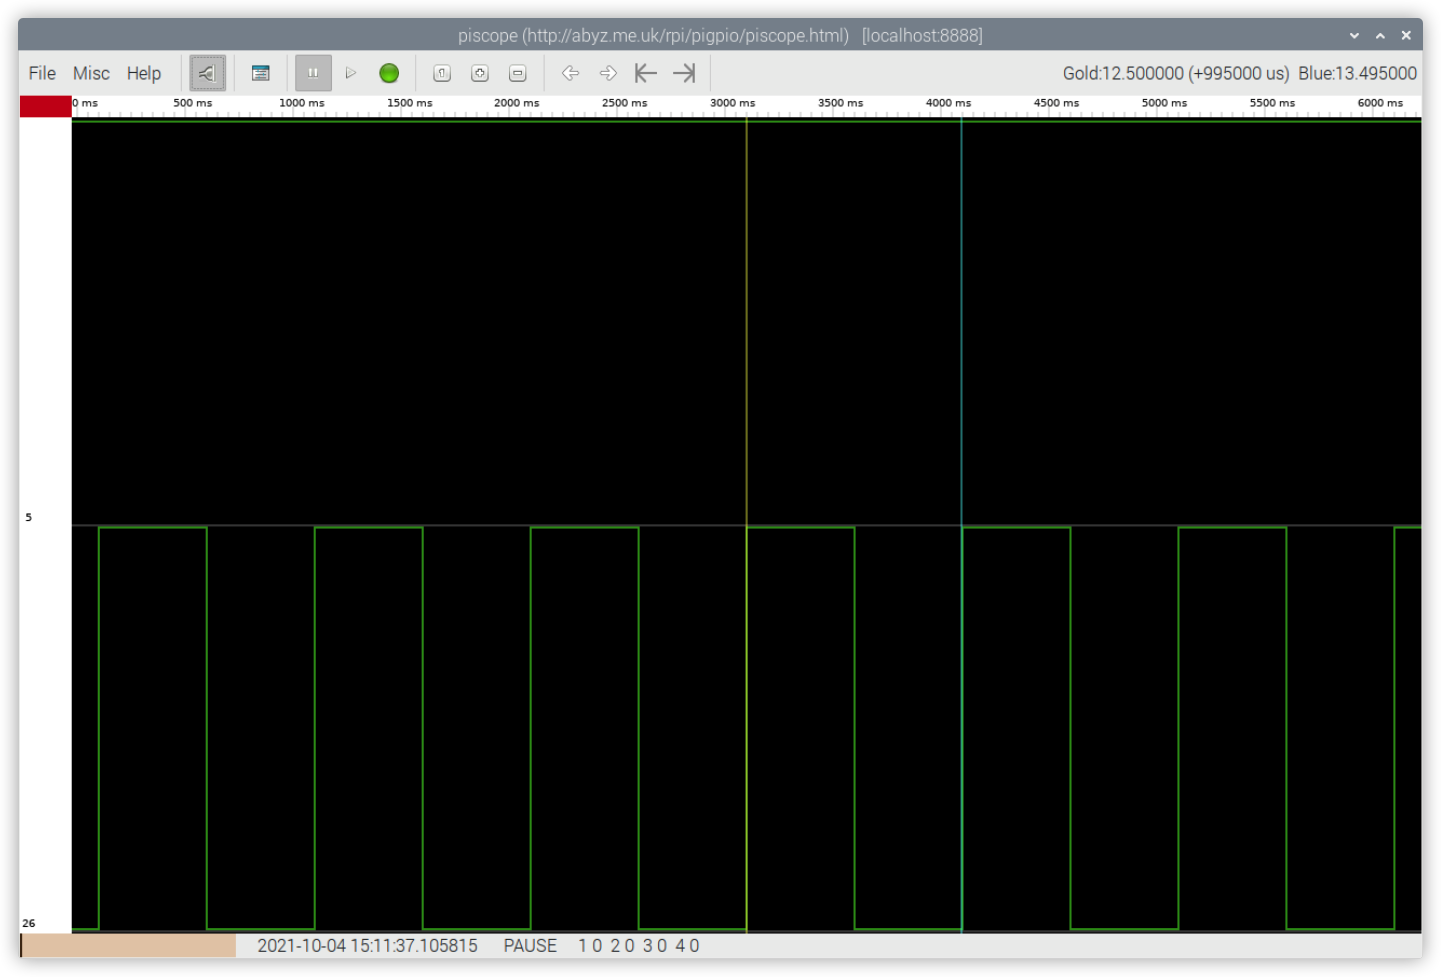
\includegraphics[width=0.7\textwidth]{img/PWM1.png}
    \caption{PWM wave}
    \label{fig:figure1}
\end{figure}\vspace{-2em}
\subsection*{2.2 DC Motor Control}\vspace{-1em}
After mastering the method of generating and controlling PWM wave, I can start using PWM wave to control the DC motor. Following the steps in the experiment instruction guide, I completed the circuit connection step by step and designed two programs, \code{motor\_control.py} and \code{two\_wheels.py}, to test whether my circuit is correct.\par
The circuit part is a little bit tricky but it's not that difficult except for one thing that I want emphasize here. At the beginning, we only need to control one DC motor. But in the subsequent process, we need to add another DC motor. This means that, in order to complete the subsequent programming, we need not only a set of PWM output, but also need another set of PWM output to control another DC Motor. Therefore, we need to use the B set on the motor controller. I didn't understand this when I first did this part of the experiment. So my first \code{two\_wheel.py} program couldn't let two DC Motors running together. After TA's reminder, I understood that it turned out that two sets of PWMs were needed to control two DC Motors, respectively. The final circuit diagram and the actual circuit are shown in figure \ref{fig:fig2} and figure \ref{fig:fig3}.
\begin{figure}[H]
\centering
\begin{minipage}[t]{0.48\textwidth}
\centering
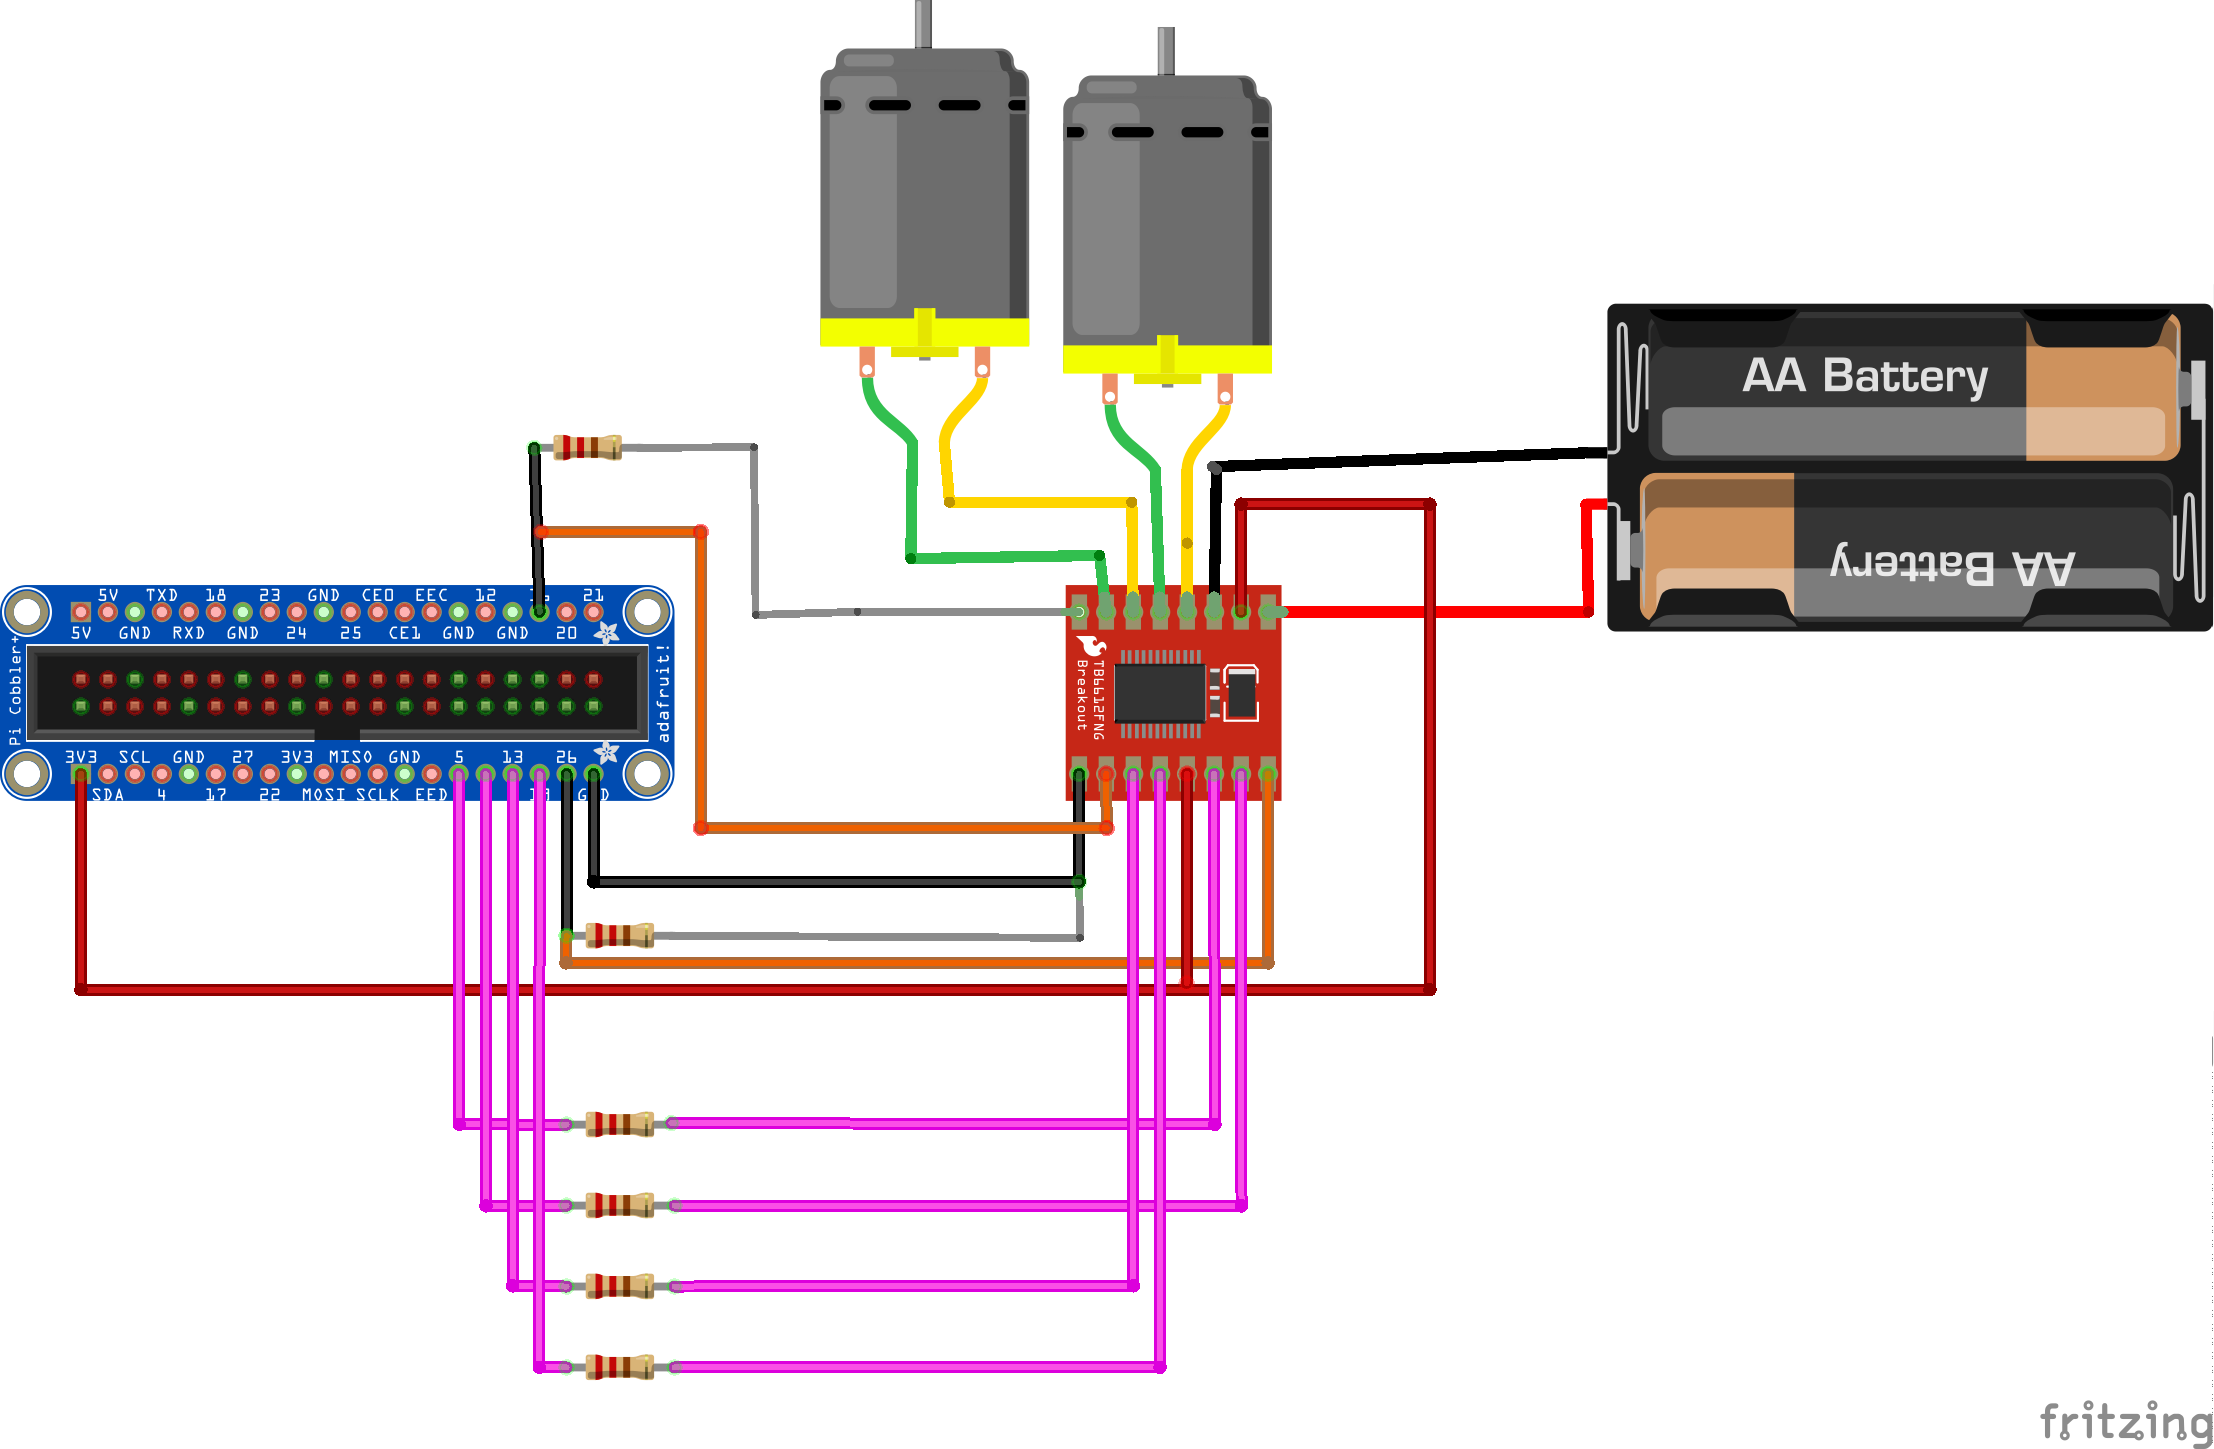
\includegraphics[width=\textwidth]{img/CircuirDiagram.png}
\caption{The circuit diagram}
\label{fig:fig2}
\end{minipage}
\begin{minipage}[t]{0.48\textwidth}
\centering
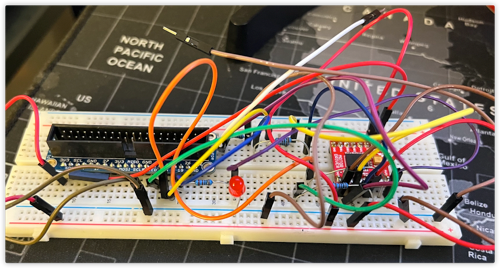
\includegraphics[width=\textwidth]{img/Circuit.png}
\caption{The actual circuit}
\label{fig:fig3}
\end{minipage}
\end{figure}
After completing the circuit design and implementation, I moved to designing programs and implementation. The complete code of \code{motor\_control.py} and \code{two\_wheels.py} have been listed in the Appendix.\par 
From essentially, the two program, \code{motor\_control.py} and \code{two\_wheels} are actually not too much difference. The only difference is that they have different methods of control. The \code{motor\_cont}\\\code{rol.py} controls the movement of the DC motor by timing while the \code{two\_wheels.py} controls the movement of two DC motors by callback functions of physical buttons. As I have already covered the code for these control logic in the previous Lab, I will not go into detail here. Instead, I want to focus more on the code for the motion logic of the DC motor. \par
The first question is how to make the DC motor run. When I was doing my experiments, this was the problem that bothered me the most. I did not know how to make the DC motor start running. At that time the TA told me the solution to the problem. Let the two GPIO pins connected to INA1 and INA2, one output high and one output low. With the voltage difference, the DC motor will turn clockwise. The example code is shown in the code listing \ref{code:code2}. I use the GPIO 26 pin as the source of PWM, the GPIO 5 ping and the GPIO 6 pin as the input of the DC motor.\par
\begin{center}
\begin{lstlisting}[language=Python, label=code:code2, caption=Example code of clockwise] 
servo_pin = GPIO.PWM(26, 1)
servo_pin.start(0)
time.sleep(2)
# Clockwise
GPIO.output(5, GPIO.HIGH)
GPIO.output(6, GPIO.LOW)
\end{lstlisting}
\end{center}\vspace{-2em}
Based on the same reason, if we flip the voltages of the two GPIO pins, the DC motor will turn counterclockwise. The example code is shown in the code listing \ref{code:code3}.
\begin{center}
\begin{lstlisting}[language=Python, label=code:code3, caption=Example code of counter-clockwise] 
# Counter-Clockwise
GPIO.output(5, GPIO.LOW)
GPIO.output(6, GPIO.HIGH)
\end{lstlisting}
\end{center}\vspace{-2em}
What's more, if we let  both output of two GPIO pin to be low, the DC motor will stop. The example code is shown in the code listing \ref{code:code4}. \par 
\begin{center}
\begin{lstlisting}[language=Python, label=code:code4, caption=Example code of stop] 
# Stop
GPIO.output(5, GPIO.LOW)
GPIO.output(6, GPIO.LOW)
\end{lstlisting}
\end{center}\vspace{-2em}
So what is the role of PWM waves? After trying to change the frequency and duty cycle of the PWM, I realised that we were changing the speed of the DC motor by means of the PWM wave. The higher the frequency, the faster the DC motor spins. And at the same frequency, a higher duty cycle will make the DC motor turn faster.\par
It was until at this point that I finally understood the meaning of the hardware connection. Each set of DC motor requires a PWM source input and two voltage input. The PWM wave controls the speed and the two voltage input control the direction of the motion.\par
Once I know how to control the DC motor, the rest of the code is easy to write. For \code{two\_wheels.py}, more GPIO pins are needed and the control logic will be covered in later sections, so it will not be expanded here.\par
So far, I have completed all content of week1. There were some stumbles and bumps in the process of doing the experiments, but I still managed to finish them on time.\vspace{-1em}
\subsection*{2.3 Rolling Control}\vspace{-1em}
The first requirement of week 2 is to implement a program, named as \code{rolling\_control.py}, which controls two DC controller and simultaneously display log history on the piTFT screen. The implementation of this program is not really difficult, but it is essential to have a framework which is easy to extend and stable. We can divide the code of this program into two parts: the piTFT screen display and updating the content, and the button callbacks and control of the DC motor. The logic of the first part of the code is similar to the Pygame program we implemented in Lab2. And the code logic for the second part is similar to that of \code{two\_wheels.py} in the previous section. Next, I will present my programming design one by one according to different topics.\par
Firstly I would like to introduce my design for the content displayed on the piTFT screen and how to update the content after event happened. The interface I ended up with is shown in the figure \ref{fig:fig4}. This interface consists of 3 parts: history, "Panic Stop" button and the "Quit" button. 
\begin{figure}[H]
    \centering
    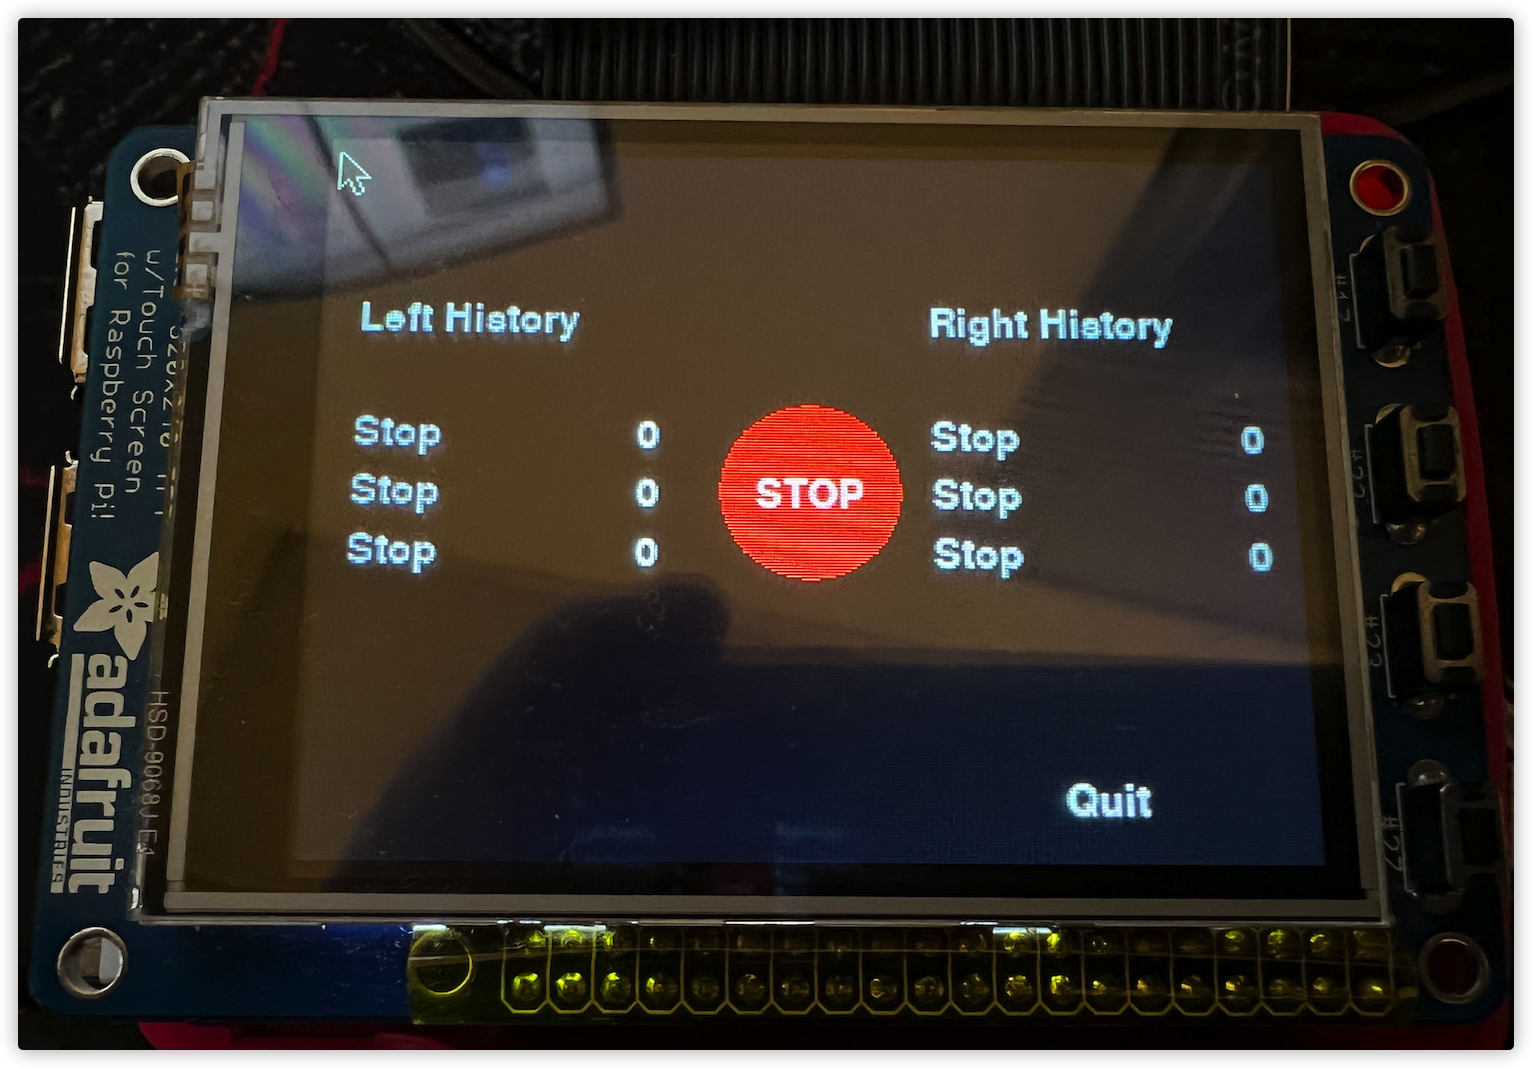
\includegraphics[width=0.7\textwidth]{img/RollingControl.png}
    \caption{The interface of rolling\_control.py}
    \label{fig:fig4}
\end{figure}\vspace{-2em}
The purpose of the history section is to hold the records and times of the three most recent operations on the left and right wheels. The function of the "Panic Stop" button is to stop the left and right wheels as soon as it is pressed. Pressing this button again will return the left and right wheels to the state they were in before they were stopped. And the function of the "Quit" button is terminating the entire program.\par
To implement the history section, I have stored the operation history of the left and right sides separately in a dictionary. To ensure that each operation will be recorded and updated immediately, I have designed a function that updates the log. This function,\code{upload\_log(side, event\_type, el}\\\code{apse\_time)} , will be called after each button press and then save newest operation event to the corresponding history dictionary. The example code is shown in the code listing \ref{code:code5}.
\begin{center}
\begin{lstlisting}[language=Python, label=code:code5, caption= Update log history] 
left_log_dict = {(10, 100): ["Stop", "0"], (10, 120): ["Stop", "0"], (10, 140): ["Stop", "0"]}
right_log_dict = {(220, 100): ["Stop", "0"], (220, 120): ["Stop", "0"], (220, 140): ["Stop", "0"]}

def upload_log(side, event_type, elapse_time):
    if side == 'left':
        print("Update the left_log")
        log_dict = left_log_dict
        has_dict = left_log_position_hash_dict
    else:
        print("Update the right_log")
        log_dict = right_log_dict
        has_dict = right_log_position_hash_dict
    log_dict[has_dict[3]] = log_dict[has_dict[2]]
    log_dict[has_dict[2]] = log_dict[has_dict[1]]
    log_dict[has_dict[1]] = [event_type, str(int(elapse_time))]
    print(log_dict)
    print('\n')
\end{lstlisting}
\end{center}\vspace{-2em}
The implementation of the "Quit" button is every straightforward. As with the logic of our previous “Quit" button design, a global bool variable \code{CODERUN} is used to determine whether to continue running the program. When the "Quit" button is pressed, \code{CODERUN} is changed to false to achieve the exit effect.\par
For me, the hardest part of the whole program was the design and implementation of the "STOP" button, because I kept misunderstanding the meaning of the resume process. After several discussions with the TA and the professor, I finally understood that resume means to return both wheels to the state they were in before the "STOP" button was pressed. With this in mind, it was easy to implement the "STOP" function. For the left and right wheels, I have designed a resume function that reads the second state of the operation in the history dictionary of the left and right wheels, which is also the state before the "STOP" button was pressed, and then rewrites this state into the corresponding history dictionary so that it is the most recent state. The code of these resume functions are shown in the code listing \ref{code:code6}.
\begin{center}
\begin{lstlisting}[language=Python, label=code:code6, caption= Resume Functions] 
def resume_left():
    global  left_log_dict, left_log_position_hash_dict
    left_last_command = left_log_dict[left_log_position_hash_dict[2]][0]
    print(left_last_command)
    if left_last_command == "Stop":
        left_wheel_stop()
    elif left_last_command == "Counter-Clk":
        left_wheel_counterclockwise()
    elif left_last_command == "Clkwise":
        left_wheel_clockwise()

def resume_right():
    global right_log_dict, right_log_position_hash_dict
    right_last_command = right_log_dict[right_log_position_hash_dict[2]][0]
    print(right_last_command)
    if right_last_command == "Stop":
        righ_wheel_stop()
    elif right_last_command == "Counter-Clk":
        right_wheel_counterclockwise()
    elif right_last_command == 'Clkwise':
        right_wheel_clockwise()
\end{lstlisting}
\end{center}\vspace{-2em}
Next, I would like to introduce all the GPIO pins that I use and their functions. As shown in the table \ref{table: table1}, the GPIO 26 and 16 are used to generate PWM wave. The GIOP 5 and 6 pin are used for providing voltage to the left wheel. The GIOP 16 and 19 are used for providing voltage to the right wheel. The GPIO 17, 22, 23 and 27 are used to control the left wheel and the right wheel with callback functions. \vspace{-2em}
\begin{table}[H]
\centering
 \caption{GPIO pins and Corresponding Functions}
 \label{table: table1}
 \begin{tabular}{|c| c |} 
 \hline
 GPIO Pin & Function  \\ [0.5ex] 
 \hline
 26 & PWM  \\ 
 \hline
 16 & PWM \\
 \hline
 5 & Left Wheel Voltage \\
 \hline
 6 & Left Wheel Voltage \\
 \hline
  16 & Right Wheel Voltage \\
 \hline
  19 & Right Wheel Voltage \\
 \hline
 17 & Left Wheel Clockwise or Stop \\
 \hline
 22 & Left Wheel Change direction \\
 \hline
 23 & Right Wheel Clockwise or Stop\\
 \hline
27 & Right Wheel Change direction  \\ 
 \hline
 \end{tabular}
\end{table}\vspace{-2em}
To improve the reusability and stability of the code, I have written all operations on the wheel as functions. The name of these functions and their corresponding functions are listed in table \ref{table: table2}. \par
\begin{table}[H]
\centering
 \caption{Operation Functions of Wheels}
 \label{table: table2}
 \begin{tabular}{|c| c |} 
 \hline
 Function Name & Function  \\ [0.5ex] 
 \hline
 left\_wheel\_start & Start the left wheel at clockwise direction  \\ 
 \hline
 left\_wheel\_stop & Stop the left wheel \\
 \hline
 left\_wheel\_counterclockwise & Change the direction of the left wheel to counter-clockwise \\
 \hline
 left\_wheel\_clockwise & Change the direction of the left wheel to clockwise  \\
 \hline
  right\_wheel\_start & Start the right wheel at clockwise direction \\
 \hline
  righ\_wheel\_stop & Stop the right wheel  \\
 \hline
 right\_wheel\_counterclockwise & Change the direction of the right wheel to counter-clockwise  \\
 \hline
 right\_wheel\_clockwise & Change the direction of the right wheel to clockwise \\ 
 \hline
 \end{tabular}
\end{table}\vspace{-2em}
In practice, the GPIO pins mentioned in the table \ref{table: table1}, which are used to control the wheel, e.g. 17, are used to implement their functions by calling the relevant functions in table \ref{table: table2}. For example, in order to change the direction of the left wheel, the callback function of the GPIO 22 pin will call the function \code{left\_wheel\_counterclockwise} and the function \code{left\_wheel\_clockw}\\\code{ise}. The example code is shown in the code listing \ref{code:code7}.\par
\begin{center}
\begin{lstlisting}[language=Python, label=code:code7, caption= Example implementation of GPIO 22 pin] 
def resume_left():
    global  left_log_dict, left_log_position_hash_dict
    left_last_command = left_log_dict[left_log_position_hash_dict[2]][0]
    print(left_last_command)
    if left_last_command == "Stop":
        left_wheel_stop()
    elif left_last_command == "Counter-Clk":
        left_wheel_counterclockwise()
    elif left_last_command == "Clkwise":
        left_wheel_clockwise()

def resume_right():
    global right_log_dict, right_log_position_hash_dict
    right_last_command = right_log_dict[right_log_position_hash_dict[2]][0]
    print(right_last_command)
    if right_last_command == "Stop":
        righ_wheel_stop()
    elif right_last_command == "Counter-Clk":
        right_wheel_counterclockwise()
    elif right_last_command == 'Clkwise':
        right_wheel_clockwise()
\end{lstlisting}
\end{center}\vspace{-2em}
After the logic of these parts has been well designed, it is not far from implementing the full requirements of this code. The complete code of \code{rolling\_control.py} is shown in the Appendix.

\subsection*{2.4 Robot Assembly and Run Test}\vspace{-1em}
In this final section, three things need to be accomplished. The first is to assemble our robot. implement \code{run\_test.py} on the basis of \code{roll\_controlling.py}. Finally modify the raspberry pi booting file to let the \code{run\_test.py} automatically run after booting the device.\par
It is not very difficult for assembling a robot. But because I am doing it alone, it will take a little more work. There are two points to note.The first thing is to be careful not to mount the DC motor upside down when installing it. The second is that care needs to be taken in the design to distribute the weight evenly so that there is not too much weight on the rear of the car. This can cause the car to lean back and not be able to go straight.\par
There's not much to say about the last step. I followed the steps in the guide very well.The only problem is that sometimes the touchscreen does not respond after a reboot. The solution is to call the \code{fix\_touchscreen} script provided by the professor earlier before the \code{run\_test.py}. This ensures that the touchscreen is available before the program run. Next I'd like to elaborate on the biggest problem I encountered while designing \code{run\_test.py}.\par
The question is how to design the timing mechanism of this program. At first, following my previous experience, I simply used the \code{time.sleep()} function. But when the professor checked, he found that the \code{time.sleep()} function would block the response to my "STOP" button as the program was sleeping.\par
The solution to this problem is actually quite simple. It is to use a global counter to manually simulate a clock. At the end of each loop the counter is incremented by 1. And in the function that detects the event, the value of the counter at this point is used to determine which event is currently in the time phase.\par
Apart from this, there is one more point that needs to be explained. In the \code{run\_test.py}, the robot needs to be controlled to do four actions: go forward, go backward, turn left and turn right. In order to implement these functions we need to know how the wheels of the robot move in each movement. The logic of my design is shown in the table \ref{table: table2}. The clockwise and counter-clockwise in the table also relate to the direction in which the DC motor is connected to the motor controller. \par
\begin{table}[H]
\centering
 \caption{State of Wheels for Each Kind of Motion}
 \label{table: table2}
 \begin{tabular}{|c| c| c |} 
 \hline
 Motion & Left Wheel & Right Wheel  \\ [0.5ex] 
 \hline
 Move Forward &  Clockwise &  Clockwise\\ 
 \hline
 Move Backward &  Counter-Clockwise &  Counter-Clockwise\\ 
 \hline
 Pivot Left & Clockwise &  Counter-Clockwise\\
 \hline
 Pivot Right & Counter-Clockwise &  Clockwise\\
 \hline
 \end{tabular}
\end{table}\vspace{-2em}
Because I have written out the functions for each type of movement separately in the \code{rolling\_contro}\\\code{l.py}, I can directly call these functions to implement these motion states. The example code is shown in the code listing \ref{code:code8}.
\begin{center}
\begin{lstlisting}[language=Python, label=code:code8, caption= Example Implementation of Motion Control] 
def move_forward():
    left_wheel_clockwise()
    right_wheel_clockwise()
    
def move_backword():
    left_wheel_counterclockwise()
    right_wheel_counterclockwise()

def stop():
    left_wheel_stop()
    righ_wheel_stop()

def pivot_right():
    left_wheel_clockwise() 
    right_wheel_counterclockwise()

def pivot_left():
    left_wheel_counterclockwise()
    right_wheel_clockwise()
\end{lstlisting}
\end{center}\vspace{-2em}
Once these two problems have been solved, it is very easy to fulfil all the requirements. The complete code of \code{run\_test.py} is shown in the Appendix.\vspace{-1em}
\section*{3. Conclusion}\vspace{-1em}
Although I didn't finish this experiment very quickly, I believe it was probably my favourite ont of the 4 experiments. Not only is there a rich hardware part, but also the software needs to be designed according to the hardware and requirements. In the process of completing this experiment, I refactored and optimised my software architecture twice. Having a highly scalable framework made it very easy for me to complete subsequent code. Bugs could be found and fixed within minutes. The only problem was that I was a bit slow in completing the hardware part because I was solo. Installing the DC motor is very unfriendly for one person. \par
Finally, I would like to thank the professors and all the TAs who were very helpful during the experiment. 

\newpage
\section*{4. Code Appendix\vspace{-1em}}
\begin{center}
\lstinputlisting[language=Python, caption=blink.py]{code/blink.py}
\end{center}\vspace{-2em}

\begin{center}
\lstinputlisting[language=Python, caption=motor\_control.py]{code/motor_control.py}
\end{center}\vspace{-2em}

\begin{center}
\lstinputlisting[language=Python, caption=two\_wheel.py]{code/two_wheel.py}
\end{center}\vspace{-2em}

\begin{center}
\lstinputlisting[language=Python, caption=rolling\_control.py]{code/rolling_control.py}
\end{center}\vspace{-2em}

\begin{center}
\lstinputlisting[language=Python, caption=run\_test.py]{code/run_test.py}
\end{center}\vspace{-2em}



% To add math, use
%\begin{equation}
 %Helpful links    https://www.overleaf.com/learn/latex/Mathematical_expressions
%\end{equation}

%To add hyperlinks, use 
%For further references see \href{http://www.overleaf.com}{Something Linky} or go to the next url: \url{http://www.overleaf.com}

% It's also possible to link directly any word or \hyperlink{thesentence}{any sentence} in you document.

% Tables 

% \begin{table}[h!]
% \centering
%  \begin{tabular}{||c c c c||} 
%  \hline
%  Col1 & Col2 & Col2 & Col3 \\ [0.5ex] 
%  \hline\hline
%  1 & 6 & 87837 & 787 \\ 
%  2 & 7 & 78 & 5415 \\
%  3 & 545 & 778 & 7507 \\
%  4 & 545 & 18744 & 7560 \\
%  5 & 88 & 788 & 6344 \\ [1ex] 
%  \hline
%  \end{tabular}
% \end{table}

% Images

% upload your images to the img folder. To print them in the document, uncomment the following
% \begin{figure}[h]
%     \centering
%     \includegraphics[width=0.25\textwidth]{/img/YourImageTitle}
%     \caption{a nice plot}
%     \label{fig:mesh1}
% \end{figure}

% As you can see in the figure \ref{fig:mesh1}, the 
% function grows near 0. Also, in the page \pageref{fig:mesh1} 
% is the same example.
\newpage
\printbibliography

\end{document}
